
\documentclass[12pt]{amsart}
\usepackage{geometry} % see geometry.pdf on how to lay out the page. There's lots.
\geometry{a4paper} % or letter or a5paper or ... etc
\usepackage{graphicx}
% \geometry{landscape} % rotated page geometry

% See the ``Article customise'' template for come common customisations

\title{ Space is the Place: How Dispersal and Competition Shape Genetic Variation in Continuous Space }
\author{C. J. Battey, Peter Ralph, Andrew Kern}
\date{November 2018} % delete this line to display the current date

%%% BEGIN DOCUMENT
\begin{document}

\maketitle
\tableofcontents

\section{Abstract}

\section{Introduction} %Edit away!

\section{Methods}
\subsection{ A Forward-Time Model of Evolution in Continuous Space }

\subsubsection{ Mating and Dispersal } 

\subsubsection{ Competition } 

\subsubsection{ Boundary Conditions } 

\subsubsection{ Tree Sequence Recording } 

\subsection{ Summary Statistics } 

\subsection{ Demographic Modeling }

\subsection{ Association Tests } 


\section{Results}

\subsection{ Summary Statistics }

\subsection{ Impacts on Demographic Inference and GWAS }

\subsection{ Estimating Model Parameters with Machine Learning }


\section{ Discussion } 

\section{Figures}


\begin{figure}[h]
	\centerline{
	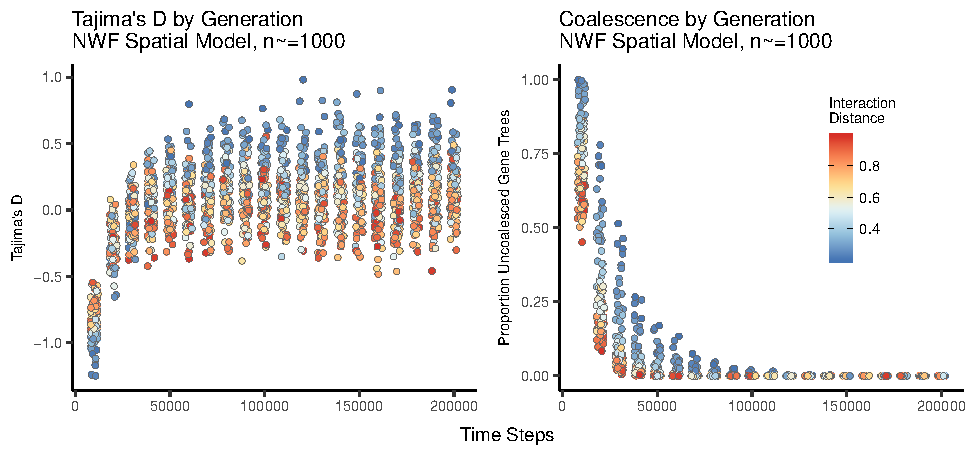
\includegraphics{../figures/10kouts_coalescence_by_generation}
	}
\end{figure}


\begin{figure}[h]
	\centerline{
	\includegraphics{../figures/sumstat_by_neighbors_spat_v_rm.pdf}
	}
\end{figure}

\begin{figure}[h]
	\centerline{
	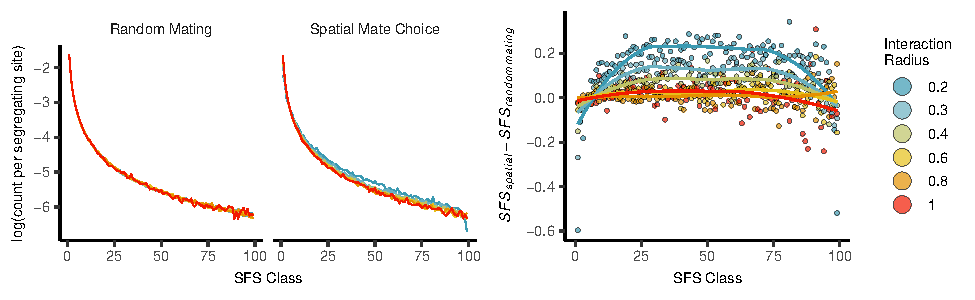
\includegraphics{../figures/sfs_spatial_v_rm.pdf}
	}
\end{figure}


\end{document}